\chapter{Asymmetrische Authentifikation von Nachrichten}
\label{cha:asymmauth}

Wie wir bereits bei den Verschlüsselungsverfahren festgestellt haben, weisen symmetrische Verfahren einige Unbequemlichkeiten auf. Allen voran stellt sich das Problem der Schlüsselverteilung, wenn für die Kommunikation zwischen zwei Partnern bei beiden derselbe Schlüssel vorhanden sein muss. Dieses Problem stellt sich natürlich umso mehr, wenn wir über einen nicht vertrauenswürdigen Kanal kommunizieren. Selbst für die Authentifikation unserer Nachrichten, die wir im Zweifelsfall nur betreiben, weil wir dem Kanal nicht vertrauen, müssen wir unter einigem Aufwand Schlüssel mit unseren Kommunikationspartnern festlegen.

Weiterhin ermöglicht symmetrische Authentifikation in keiner sinnvollen Weise, dass wir von uns veröffentlichte Dokumente oder Nachrichten unterschreiben und damit die Urheberschaft für jeden nachprüfbar machen können. Zur Authentifikation des Dokuments sollte schließlich jeder befähigt sein, der sich dafür interessiert. Wenn wir mit symmetrischen Verfahren arbeiten, bedeutet das, dass wir zur Prüfung den Schlüssel herausgeben müssen, mit dem wir das Dokument signiert haben. Das bedeutet aber auch, dass jeder Interessierte nun nicht nur zur Prüfung der bereits bestehenden Signatur in der Lage ist, sondern auch eigene Signaturen erstellen kann. Damit ist die Urheberschaft einer Unterschrift nicht mehr gesichert.

Es bietet sich ein Verfahren an, bei dem die Prüfung einer Signatur nicht mit einem privaten Schlüssel erfolgt. Dieses System kennen wir bereits aus dem Kapitel \ref{ch:asymmenc}. Bei der Verwendung von asymmetrischen Verfahren zur Authentifikation verwenden wir die folgenden Algorithmen:
\begin{itemize}
  \item \textbf{Schlüsselgenerierung:} $(pk, sk) \leftarrow \keygen(1^k)$
    \begin{itemize}
      \item $pk$ : öffentlicher Schlüssel
      \item $sk$ : privater Schlüssel
      \item $k$ : Sicherheitsparameter
    \end{itemize}
  \item \textbf{Signieren:} $\sigma \leftarrow \sig(sk,M)$
  \item \textbf{Verifizieren:} $\ver(pk,M,\sigma) \in \{ 0,1 \}$
\end{itemize}
$\sig$ und $\ver$ müssen korrekt sein, d.h. es muss wie bei MACs gelten:
\begin{equation*}
    \forall (pk,sk) \leftarrow \keygen(1^k), \forall M, \forall \sigma \leftarrow \sig(sk,M) : \ver(pk,M,\sigma) = 1
\end{equation*}
Wir passen außerdem die Definition der EUF-CMA-Sicherheit aus Abschnitt
\ref{ch:symauth:sicherheit} an asymmetrische Verfahren an.

\begin{definition}
Sei \A~ ein PPT-Algorithmus.
\begin{enumerate}
\item \A~erhält Zugriff auf ein Signarorakel $\sig(sk, \cdot)$ sowie den
  entsprechenden öffentlichen Schlüssel $pk$.
\item \A~darf nun polynomiell viele Nachrichten $\plaint_i$ an das
  Orakel schicken und erhält $\sigma_i \leftarrow \sig(sk, \plaint_i)$ als Antwort.
\item \A~gibt als (potentielle) Fälschung ein Nachrichten-Signatur-Paar
  $(\plaint^*,\sigma^*)$ aus.
\item \A~gewinnt, wenn $\sigma^*$ eine gültige Signatur für
  $\plaint^*$ ist, d.h. $\ver(\pkey, \plaint^*, \sigma^* = 1)$, und $\plaint^*
  \neq \plaint_i$ für alle $i$ ist, d.h. $\plaint^*$ nicht zu den
  Nachrichten gehört, die sich \A~vom Orakel hat signieren lassen.
\end{enumerate} 

Ein asymmetrisches Signaturverfahren ist EUF-CMA-sicher, wenn jeder
beliebige PPT-Angreifer \A~ das oben genannte Spiel nur mit im
Sicherheitsparameter $k$ vernachlässigbarer Wahrscheinlichkeit gewinnt. 
\end{definition}

Die Definition unterscheidet sich also dadurch, dass
\A~mithilfe des öffentlichen Schlüssels selbst Signaturen verifizieren kann. Anders
als im symmetrischen Fall ist also eine Unterscheidung zwischen zwei
Begriffen mit und ohne Verifikationsorakel nicht nötig. 

\section{RSA}
Wir betrachten zuerst RSA als Kandidaten für ein asymmetrisches
Signaturverfahren. Der Generatoralgorithmus für RSA-Signaturen ist
identisch zu dem für RSA-Verschlüsselung, der in Kapitel
\ref{ch:asymmenc:rsa:vorgehen} besprochen wurde:
\begin{itemize}
 	\item Wähle zwei große Primzahlen $P, Q$ mit $P \neq Q$ und vorgegebener Bitlänge $k$.
 	\item Berechne $N = P \cdot Q$.
 	\item Berechne $\varphi(N) = (P - 1)(Q - 1)$\footnote{$\varphi$
            bezeichnet die Eulersche Phi-Funktion. Sie gibt für jede
            natürliche Zahl n an, wie viele zu n teilerfremde natürliche
            Zahlen es gibt, die nicht größer als n sind: 
            $\varphi(n) := \vert \{a\in\N \, |\, 1 \le a \le n
            \land \operatorname{ggT}(a,n) = 1 \} \vert$. Insbesondere
            ist $\varphi(N)$ die Anzahl multiplikativ invertierbarer
            Elemente im Restklassenring $\mathbb{Z}/N\mathbb{Z}$.
            Sie ist multiplikativ, d.h. es gilt für teilerfremde $n$, $m$:
            $\varphi(m\cdot n) = \varphi(m) \cdot \varphi(n)$. Da eine
            Primzahlen $p$ nur durch 1 und sich selbst teilbar ist, 
            gilt $\varphi(p) = p-1$. Somit gilt für zwei Primzahlen $p$,
            $q$ also $\phi(p \cdot q) = \phi(p) \cdot \phi(q) = (p-1)(q-1)$.}.
 	\item Wähle $e \in \{3, \dotsc, \varphi(N) - 1\}$, wobei
          $\ggT(e, \varphi(N)) = 1$. 
 	\item Berechne mit Hilfe des \hyperref[ssec:eea]{EEA} das zu $e$
          multiplikativ-inverse Element $d$ bezüglich $\varphi(N)$,
          d.h. $d \equiv e^{-1} \pmod{\varphi(N)}$.
        \item $(pk, sk)\leftarrow ((N,e), (N,d))$.
\end{itemize}
Die Signatur- und Verifikationsalgorithmen funktionieren ähnlich wie die
Ver- und Entschlüsselungsalgorithmen aus Kapitel \ref{ch:asymmenc:rsa:vorgehen}\footnote{Oft liest man, dass das Signieren
  von Nachrichten immer dem Verschlüsseln mit dem geheimen Schlüssel
  entspricht. Dies gilt jedoch im Allgemeinen nicht. RSA ist hier eine
  seltene Ausnahme!}:
\begin{alignat*}{3}
& \sig(\skey, \plaint) & = \plaint^d & \mod N\\
& \ver(\pkey, \plaint, \sigma) & = 1 : \Leftrightarrow \plaint = \sigma^e & \mod N 
\end{alignat*}

Das Verfahren hat jedoch einige Nachteile:
\begin{description}
    \item[Signatur \glqq unsinniger\grqq~Nachrichten:] Ein Angreifer
      wählt zunächst ein beliebiges $\sigma \in \mathbbm{Z}$. Dann kann
      er mithilfe des öffentlichen Schlüssels $\pkey$ zu dieser Signatur
      einfach ein $\plaint$ generieren, zu dem die Signatur $\sigma$
      passt: $\plaint := \sigma^e \mod N$.\\ 
    Zwar ist für diesen Angriff im ersten Moment keine sinnvolle Nutzung
    ersichtlich, da der Angreifer keine Kontrolle darüber hat, für
    welche Nachricht er eine Signatur fälscht, die Problematik eines
    Missbrauchs besteht jedoch prinzipiell. Dieser Angriff bricht also
    die für ein Signaturverfahren geforderte EUF-CMA-Sicherheit.
  \item[Homomorphie von RSA:] Angenommen, ein Angreifer ist im Besitz
    zweier Signaturen $\sigma_1$, $\sigma_2$ zu den Nachrichten
    $\plaint_1$, $\plaint_2$. Dann kann er eine gültige Signatur
    $\sigma_3$ für
    eine Nachricht $\plaint_3 = \plaint_1 \cdot \plaint_2 \mod N$
    berechnen mit
    \begin{alignat*}{2}
      \sigma_3 &= \plaint_3^d  & \mod N\\
               &=  (\plaint_1 \cdot \plaint_2)^d & \mod N \\
               &= \plaint_1^d \cdot \plaint_2^d &\mod N\\
               &= \sigma_1 \cdot \sigma_2 &\mod N
    \end{alignat*}
  \end{description}
  Aus der Homomorphie kann man sich einen Angreifer bauen, der das
  EUF-CMA-Sicherheits\-experiment gewinnt: 
  \begin{beispiel}
    Sei \A~ein PPT-Algorithmus und \C~ein Challenger im
    EUF-CMA-Sicherheits\-experiment. Das Experiment läuft wie folgt ab.
    \begin{itemize}
    \item \A~wählt zwei Nachrichten $M_1$, $M_2$ so, dass $ M_1\cdot M_2
      \neq M_i \mod N$ für beide $i$, und sendet diese an \C
    \item \C~erstellt die Signaturen $\sigma_1$, $\sigma_2$ und sendet
      diese an \A
    \item \A~ berechnet $M_3=M_1M_2 \mod N$ und
      $\sigma_3=\sigma_1\sigma_2 \mod N$ und gibt diese aus.
    \end{itemize}
    Damit hat \A~eine Gültige Signatur gefälscht und gewinnt das Experiment.
  \end{beispiel}
Wie bereits bei der RSA-Verschlüsselung in Kapitel \ref{ch:asymmenc:rsa:sicherheit} können wir diese Probleme lösen, indem wir die Nachricht vor der Verarbeitung padden:
\begin{align*}
\sig(\skey,\plaint) &= (\text{pad}(\plaint))^d \mod N\\
\ver(\pkey,\sigma,\plaint) &= 1 :\Leftrightarrow \sigma^e \mod N \text{ ist gültiges Padding für } \plaint
\end{align*}
Das so entstandene Signaturverfahren nennt sich (RSA-)PSS
(\emph{Probabilistic Signature Scheme}) und ist wie RSA-OAEP (als Teil
der \emph{PKCS}) kryptographischer
Standard.\footnote{\url{http://www.emc.com/emc-plus/rsa-labs/standards-initiatives/pkcs-rsa-cryptography-standard.htm}} 
Die \textit{pad}-Funktion wird in Abb. \ref{fig:pss} dargestellt. Sie
erweitert eine Nachticht \plaint~zu einer \textit{encodet Message
  EM}. Das Verifizieren einer so gepaddeten Nachricht wird in
Abb. \ref{fig:pss-vfy} dargestellt. Eine detailierte Erläuterung des
Verfahrens erfolgt hier nicht, kann aber im RFC-Standard 3447
\footnote{\url{https://tools.ietf.org/html/rfc3447}} nachgelesen werden.

\begin{figure}[h]
  \centering
  \begin{subfigure}[b]{.45\textwidth}
    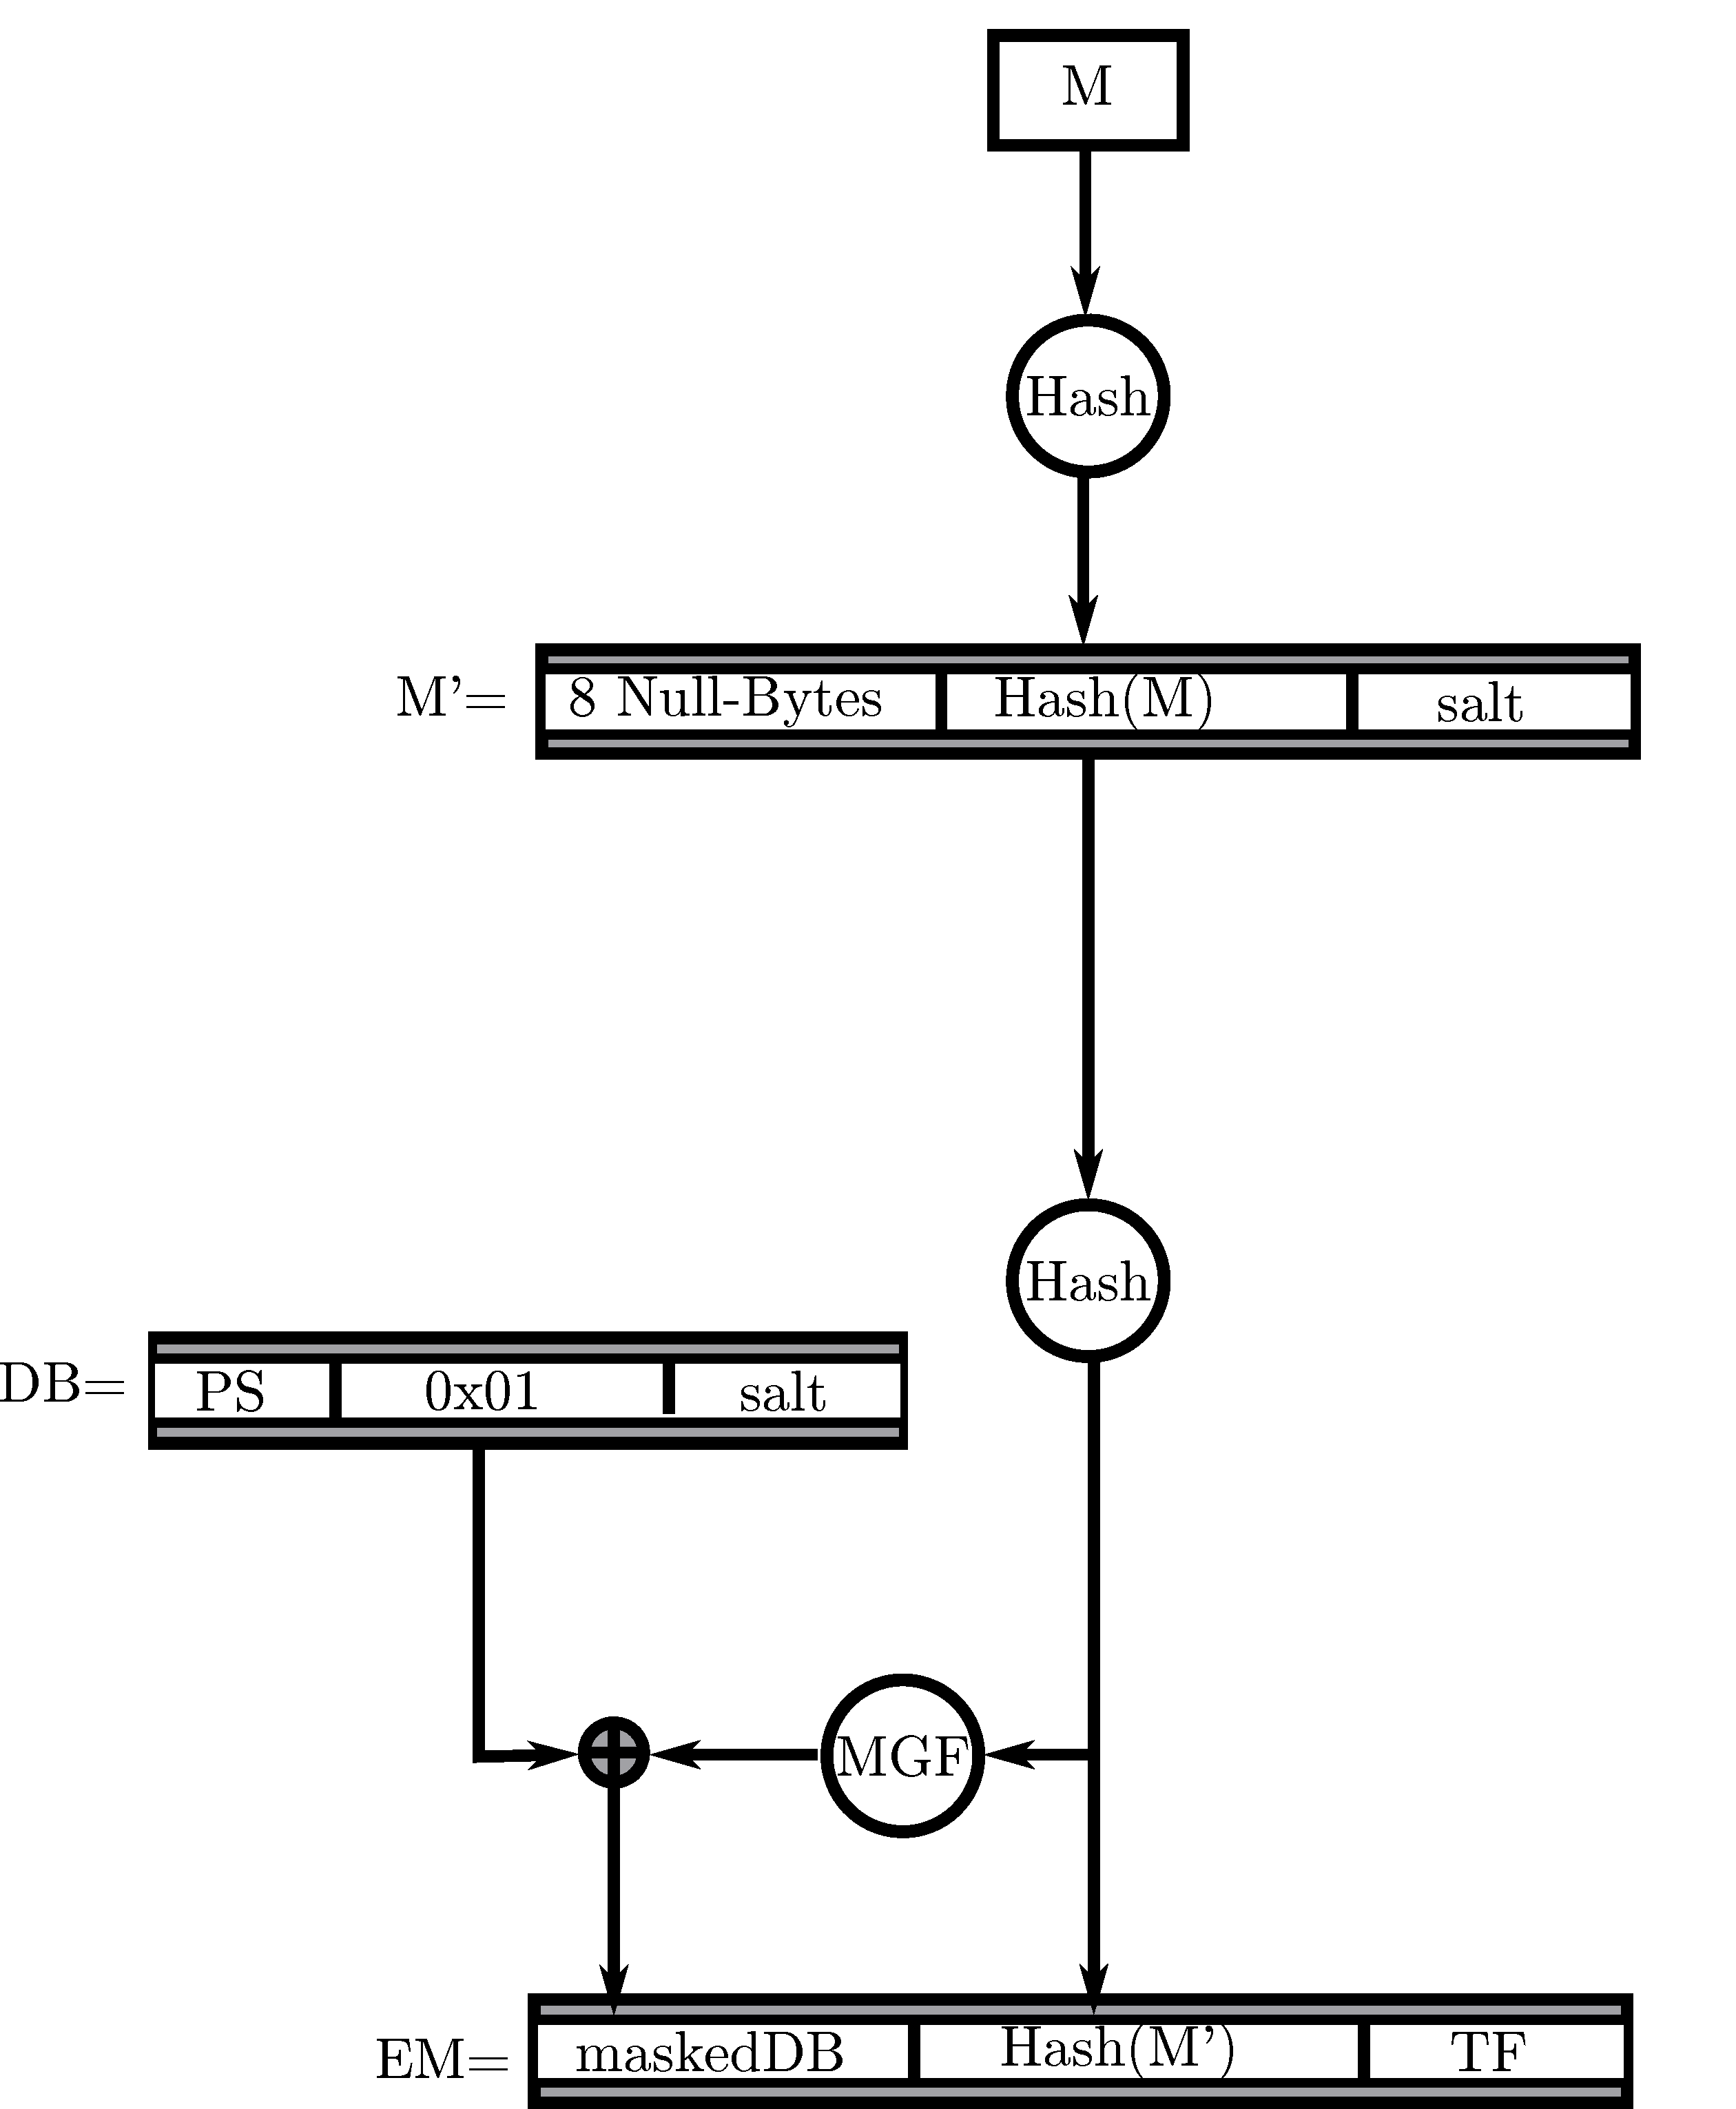
\includegraphics[width=\textwidth]{images/pss.pdf}
    \caption{Padding für RSA-PSS}
    \label{fig:pss}
  \end{subfigure}
  \begin{subfigure}[b]{.45\textwidth}
    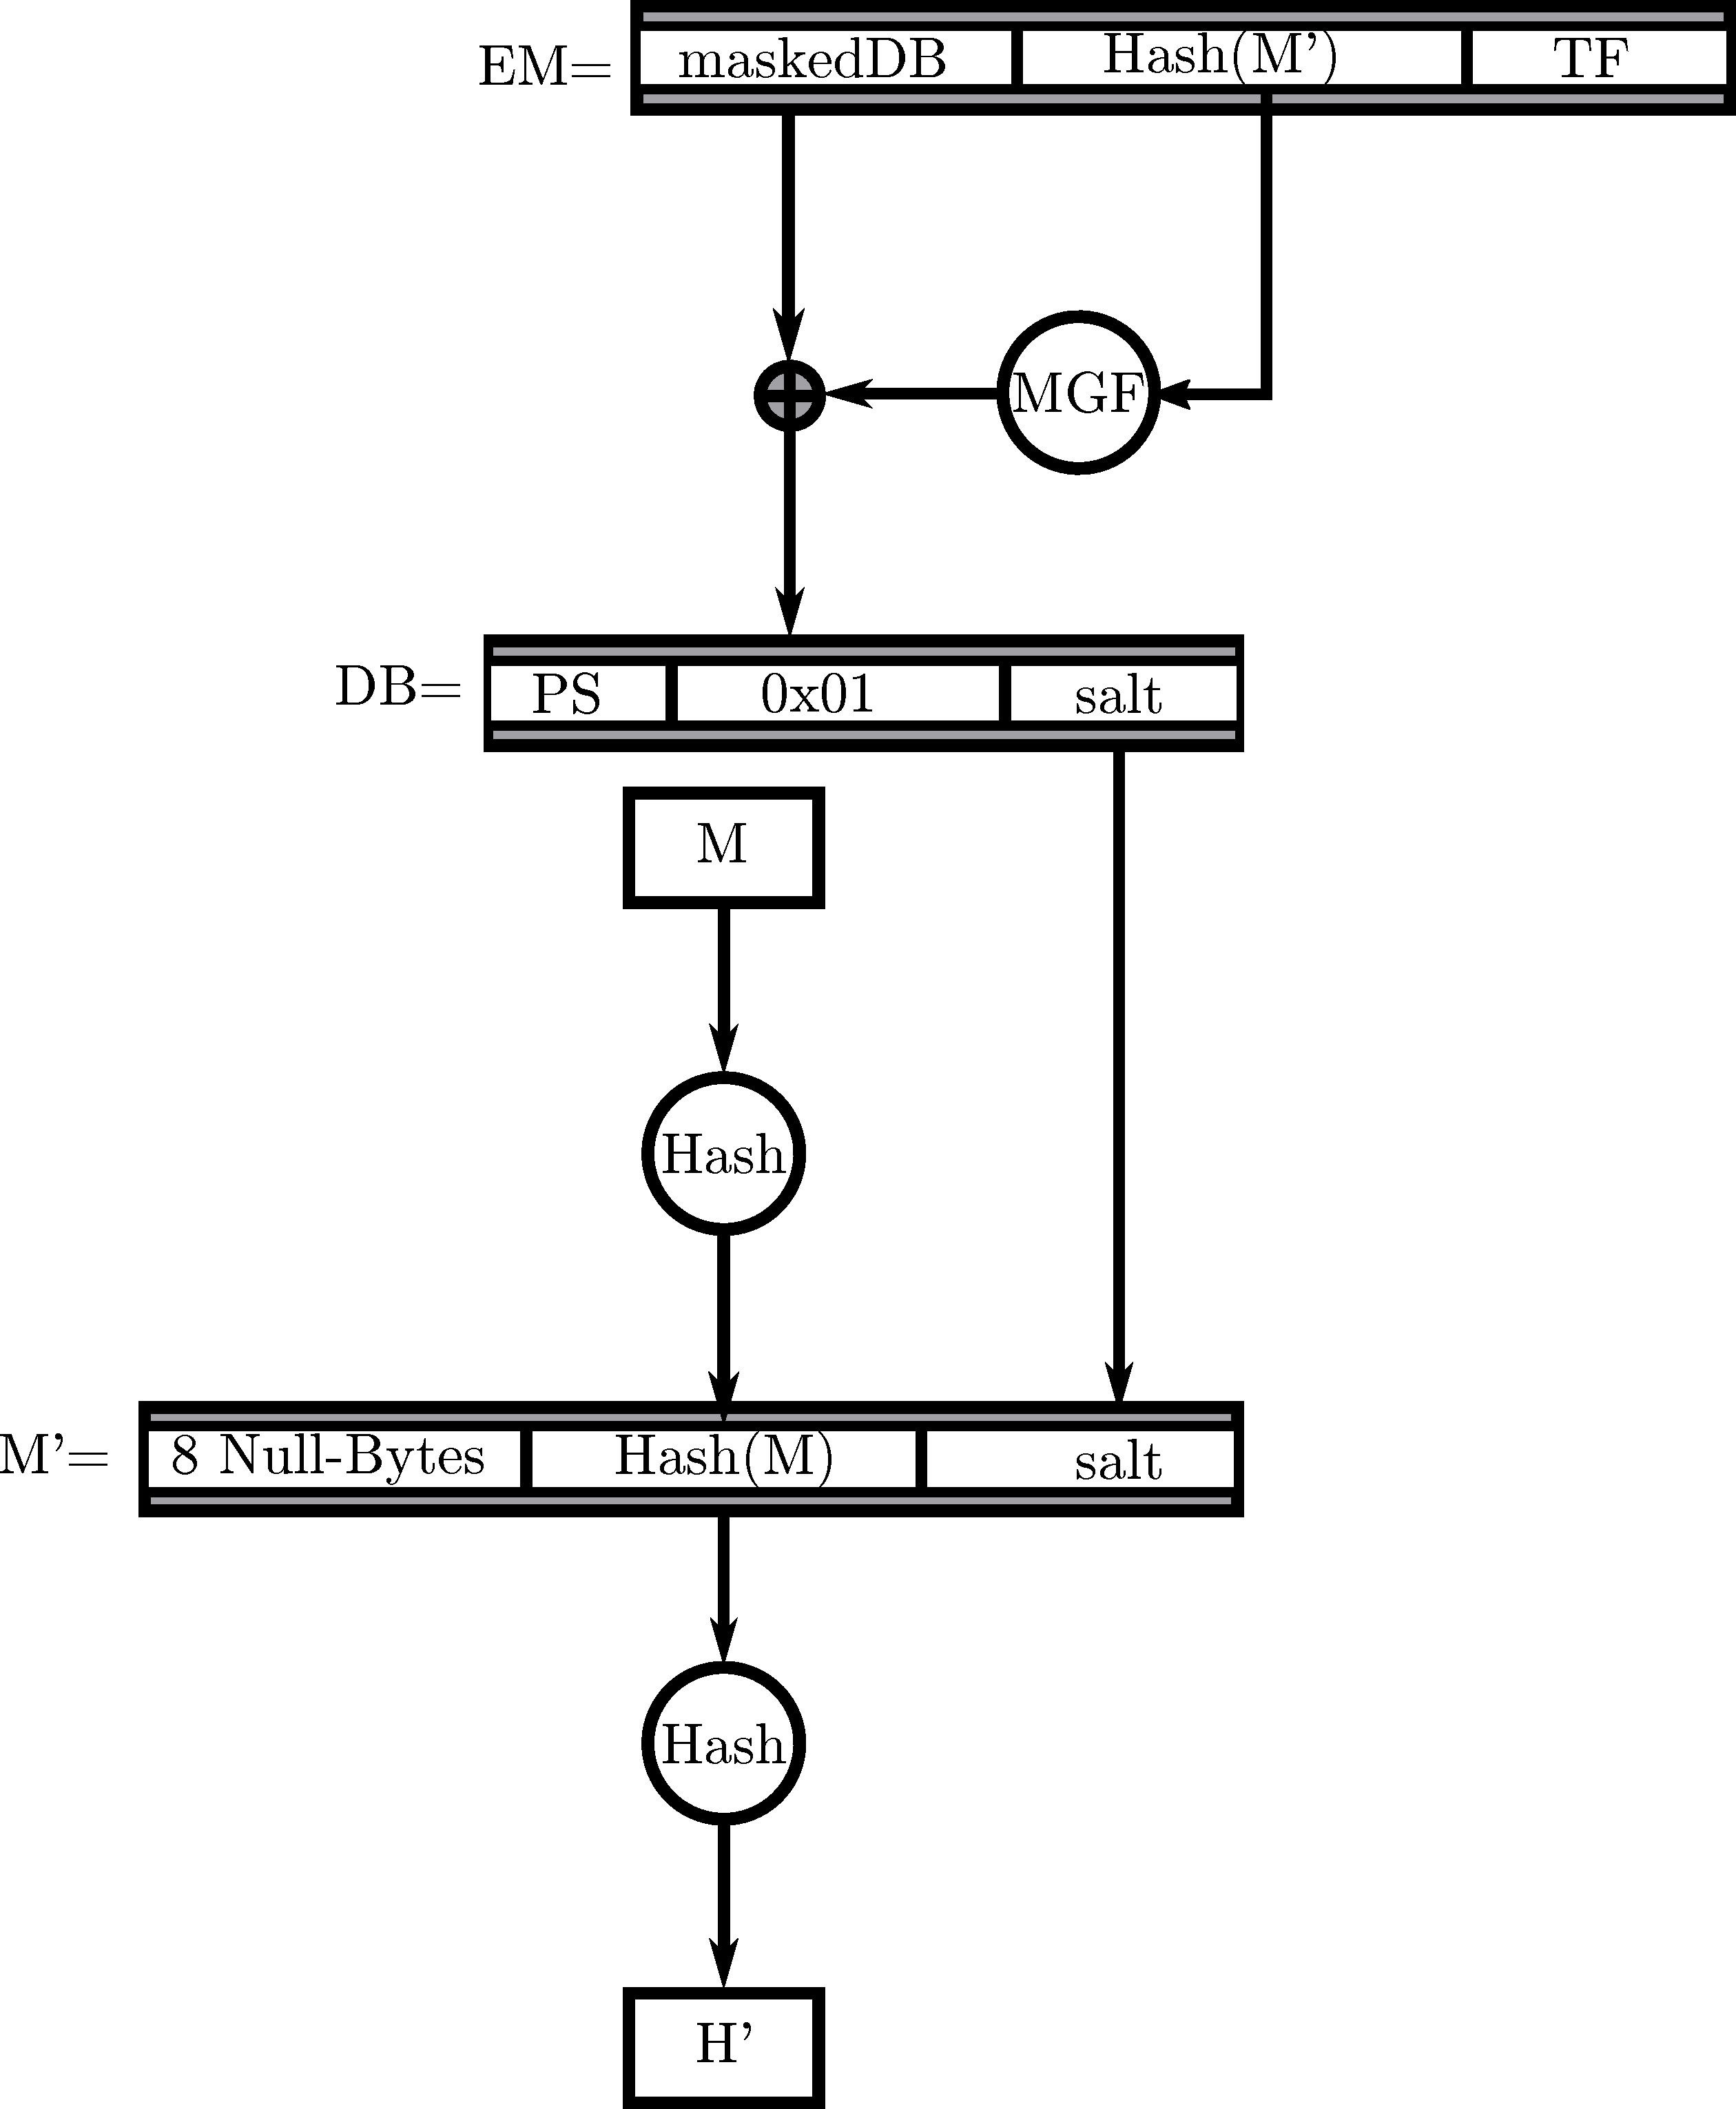
\includegraphics[width=\textwidth]{images/pss-vfy.pdf}
    \caption{Verifikation von gepaddeten Nachrichten}
    \label{fig:pss-vfy}  
  \end{subfigure}
  \caption{Ablauf der Padding-Funktion in RSA-PSS}
\end{figure}


Unter Verwendung idealer Hashfunktionen und mit der Annahme, dass die
RSA-Funktion schwierig zu invertieren ist, ist RSA-PSS heuristisch
EUF-CMA sicher\footnote{D.h. sicher im Random-Oracle-Modell}. Ein Angreifer ist gezwungen, die RSA-Funktion direkt anzugreifen. Der beste bekannte Angriff basiert auf der Faktorisierung von $N$ (unter Verwendung des Zahlkörpersiebs). Die Parameter werden ähnlich wie bei RSA-OAEP gewählt und haben so eine Länge von meistens 2048 Bit. Um eine effiziente Verifikation der Signaturen zu gewährleisten, ist es außerdem ohne Schwierigkeiten möglich, den Parameter $e$ klein zu wählen.


\section{ElGamal}
Analog zum ElGamal-Verschlüsselungssystem aus Kapitel
\ref{ch:asymenc:elgamal} betrachten wir nun ein Signaturverfahren über
der Gruppe $\G = \Z{p}^*$.
\subsection{Erste Idee}
Sei für unseren ersten Versuch der geheime Schlüssel $\skey = (\G, g,
x)$ und der öffentliche Schlüssel $\pkey = (\G, g, g^x)$. Dann bietet
sich die Verwendung von ElGamal zur Erzeugung einer Signatur auf diese
Art an: 
\begin{align*}
\sig(\skey,M) &= a \text{ mit } a \cdot x = M \mod \left|\G\right|\\
\ver(\pkey,\sigma,M) &= 1 :\Leftrightarrow (g^x)^a = g^M
\end{align*}
Allerdings lässt sich diese Konstruktion auf einfache Art brechen, indem
mit $x = M a^{-1} \mod \G$ der geheime Schlüssel berechnet wird. 

\subsection{Schlüssel- und Signaturerzeugung}
Für die Schlüssel gilt weiterhin $\skey = (\G, g,
x)$, $\pkey = (\G, g, g^x)$. 
Für die Signaturerzeugung wird eine zufällige, in $\Z{p}$ invertierbare
Zahl $e \in \{1, \dots, p - 1\}$ gewählt,
wobei $p=|\G|$. Damit berechnet man 
\begin{align*}
a &:= g^e \in \G\\
b &:= (M - a \cdot x) \cdot e^{-1} \mod p
\end{align*}
$a$ wird je nach Kontext als Gruppenelement oder als Zahl interpretiert, $b$
ist eine Zahl in $\Z{p}$.  
Damit gilt $a \cdot x + e \cdot b = M$. Das Signaturverfahren ist nun
$\sig(\skey,M) = (a, b)$.

Für das Verifikationsverfahren werden nun zwei Gruppenelemente $v_1,
v_2 \in \G$ berechnet mit
\begin{align*}
  v_1 &= (g^x)^a \cdot a^b\\
  v_2 &= g^M.
\end{align*}
Das Verifikationsverfahren ist nun
\begin{align*}
\ver(\pkey,\sigma,M) = 1 : & \Leftrightarrow v_1 = v_2 \\
 &\Leftrightarrow (g^x)^a \cdot a^b = g^M \\
 &\Leftrightarrow  g^{ax} \cdot g^{be} = g^M
\end{align*}
Doch auch bei dieser Variante gibt es noch einige offene Angriffspunkte:
\begin{description}
	\item[Doppelte Verwendung von $e$:]
	Wird der zufällige Parameter $e$ mehrmals zur Erzeugung von Signaturen verwendet, kann der geheime Schlüssel $x$ aus den beiden Signaturen errechnet werden. Seien die Signaturen $(a = g^e, b, M)$ und $(a' = g^{e'} = a, b', M')$. Dann ergibt sich durch Aufaddieren und Umformen
	der Gleichungen
	\begin{align*}
	&a \cdot x + e \cdot b = M\\
	\land \quad &a \cdot x + e \cdot b' = M'\\
	\Rightarrow \quad &e = \frac{M - M'}{b - b'}
	\end{align*}
	Mit bekanntem $e$ kann wiederum auf den geheimen Schlüssel $x$
        geschlossen werden.\footnote{Im Signaturverfahren der
          Spielekonsole \textit{PlayStation 3} (PS 3) wurde dem
          Zufallsparameter $e$ ein immer gleicher Wert zugewiesen,
          wodurch der geheime Schlüssel berechnet werden konnte. Dadurch
          wurde es möglich, unautorisierte Anwendungen, wie
          \textit{gecrackte} Spiele, auf der PS 3 auszuführen. Die
          Erklärung zu diesem erfolgreichen Angriff ist
          \href{https://www.youtube.com/watch?v=4loZGYqaZ7I}{hier} zu
          finden, wobei der Angriff auf das Signaturverfahren ab Minute
          35:30 beschrieben wird.} Bei zufälliger Wahl geschieht es nur
        vernachlässigbar oft, dass zwei Mal dasselbe $e$ ausgewählt wird
        und infolgedessen ausgenutzt werden kann .
	\item[Erzeugung "`unsinniger"' Signaturen:]
	Durch günstige Wahl der Parameter ist es möglich, auch ohne Kenntnis des Schlüssels $x$ gültige Signaturen zu erzeugen. Wähle zunächst $c$
	zufällig. Setze außerdem:
	\begin{align*}
	a &:= g^cg^x = g^{c+x}\\
	b &:= -a
	\end{align*}
        Dies impliziert $e=c+x$. 
	Dann ist $(a, b)$ eine gültige Signatur zu $M$ mit
	\begin{align*}
          M &= -ac\\
            &= a \cdot x - a \cdot (c + x)\\
            &= a \cdot x + b \cdot e,\\
	\end{align*}
        denn es gilt 
        \begin{alignat*}{3}
          &&                 & (g^x)^a\cdot a^b       &= &g^M\\
          && \Leftrightarrow & g^{ax} \cdot a^{-a}     &= &g^{-ac}\\
          && \Leftrightarrow & g^{ax} \cdot (g^e)^{-a} &= &g^{-ac}\\
          && \Leftrightarrow & g^{ax-a(c+x)}            &= &g^{-ac}\\
          && \Leftrightarrow & g^{-ac}                 &= &g^{-ac}
        \end{alignat*}
      \end{description}
      \subsection{Beispiel}
      Im Folgenden werden Schlüsselerzeugung, Signieren und Verifizieren beispielhaft
      in der multiplikative Gruppe $\G = \Z{17}^{*}$ mit Ordnung $16$ gezeigt. 
      \subsubsection*{Schlüsselerzeugung}
      Es sind $\skey = (\G, g, x)$ und $\pkey = (\G, g, g^x)$. Als
      Erzeuger wird $g=3$, als Zufallszahl wird $x=11$
      gewählt. Es sind also $\skey = (\G, 3, 11)$ und $\pkey = (\G, 3,
      3^{11})\equiv (\G, 3, 7)$.
      \subsubsection*{Signieren}
      Alice will eine Nachricht $\plaint = 10$ mit $sk$ signieren. Dazu
      wählt sie einen zufälligen, modulo 16 invertierbaren Exponenten
      $e= 13$ und berechnet mit dem erw. Euklidischen Algorithmus
      $e^{-1}=5$. Dann ist $\sigma =  (a, b)$ mit 
      \begin{align*}
       a &:= g^e &\\
         &= 3^{13} \equiv 12 & \mod 17\\
       b &:= (\plaint-a  \cdot x) \cdot e^{-1} & \mod |\G|\\
          &= (10 - 11 \cdot 12) \cdot 13^{-1} & \mod 16\\
          &\equiv (10 - 11\cdot 12) \cdot 5 \equiv 14 & \mod 16
      \end{align*}
      \subsubsection*{Verifizieren}
      Es ist
      \begin{align*}
        v_1 & = (g^x)^a \cdot a^b  & \mod 17 \\
            & = 7^{12} \cdot 12^{14} & \mod 17 \\
            & \equiv 13 \cdot 15 & \mod 17 \\
            & \equiv 8 & \mod 17 \\
        v_2 & = g^M & \mod 17 \\
            &= 3^{10} & \mod 17\\
            &\equiv 8 & \mod 17\\
      \end{align*}
      also gilt $v_1=v_2$ und die Signatur ist gültig.
     

      \section{Hash-Then-Sign-Paradigma}
      Analog zum symmetrischen Fall wollen wir mithilfe des
      Hash-Then-Sign-Paradigmas Nachrichten beliebiger Länge signieren können.
      \begin{theorem}[Hash-Then-Sign-Paradigma]
        Sei $(\keygen, \sig, \ver)$ EUF-CMA-sicher und $H$ eine
        kollisionsresistente Hashfunktion. Dann ist das durch  
        \begin{align*}
          \keygen'(1^k) &= \keygen(1^k)\\
          \sig'(\skey,M) &= \sig(\skey,H(M))\\
          \ver'(\pkey,M,\sigma) &= \ver(\pkey,H(M),\sigma)
        \end{align*}
        definierte Signaturverfahren EUF-CMA-sicher.~\\
      \end{theorem}

      Der Beweis dieses Theorems verläuft analog zu \ref{ch:symauth:eufcma-beweis}.

      Die Verwendung einer kollisionsresistenten Hashfunktion ermöglicht
      eine Abwehr gegen die Erzeugung "`unsinniger"' Signaturen, denn
      die errechneten "`unsinnigen"' Klartexte müssen nun zusätzlich
      denselben Hashwert erzeugen wie die Originalnachricht. 


\section{Digital Signature Algorithm (DSA)}
Aus der Anwendung des Hash-Then-Sign-Paradigmas auf das ElGamal-Signaturverfahren entsteht unter Verwendung einer kollisionsresistenten
Hashfunktion $H$ der \emph{Digital Signature Algorithm} (DSA):
\begin{align*}
a &:= g^e\\
b &:= (H(M) - a \cdot x) \cdot e^{-1} \mod \left|\G\right|
\end{align*}
mit der Signatur $\sigma = (a,b)$.

Der DSA ist nach RSA der zweitwichtigste Signaturalgorithmus und wurde 1994 standardisiert.\footnote{Der aktuelle Standard findet sich auf \url{http://csrc.nist.gov/groups/ST/toolkit/digital_signatures.html}} Für die Bewertung von DSA wirkt sich nachteilig aus, dass für jede neue Signatur eine frische Zufallszahl gewählt werden muss (ein guter Zufallsgenerator wird also
vorausgesetzt) und dass die Verifikation einer DSA-Signatur im Vergleich zu einer RSA-Signatur mit kleinem Modulus deutlich langsamer ist.

Ob DSA EUF-CMA-sicher ist, steht noch nicht eindeutig fest.
